\section{Method: CIKD++-RT}

In this section, we present the architecture of the proposed CIKD++-RT (Contextual Information Knowledge Distillation with Residual Transformer) framework. We formulate the problem as a 6-class multimodal misinformation detection task, where the input $x = (T, I, K, R)$ consists of Text (T), Image (I), Knowledge Graph entities (K), and Relations (R), and the output $y \in \{0,1,2,3,4,5\}$. A key focus in our research is the accurate identification of Content-Knowledge (CK) inconsistency, corresponding to class 2 in the problem formulation.

Our final model, the no\_c\_emb variant, relies entirely on the cross-attention mechanism to explicitly extract visual contradiction evidence, avoiding reliance on unreliable prior scalar quantities.

\begin{figure*}[!t]
    \centering
    
\includegraphics[width=0.70\textwidth]{figures/figure_1.png}
    \caption{Overall architecture of CIKD++-RT no\_c\_emb.}
    \label{fig:architecture}
\end{figure*}

\begin{figure}[!htbp]
    \centering
    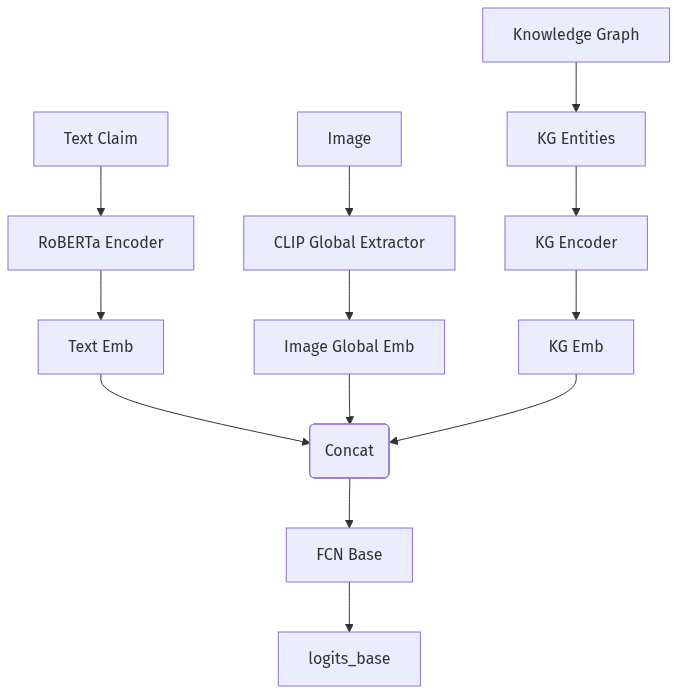
\includegraphics[width=\linewidth]{figures/figure_1_part1_passive_anchor.png}
    \caption{Passive Text+Image+KG anchor for computing logits\_base.}
    \label{fig:arch_part1}
\end{figure}

\begin{figure}[!htbp]
    \centering
    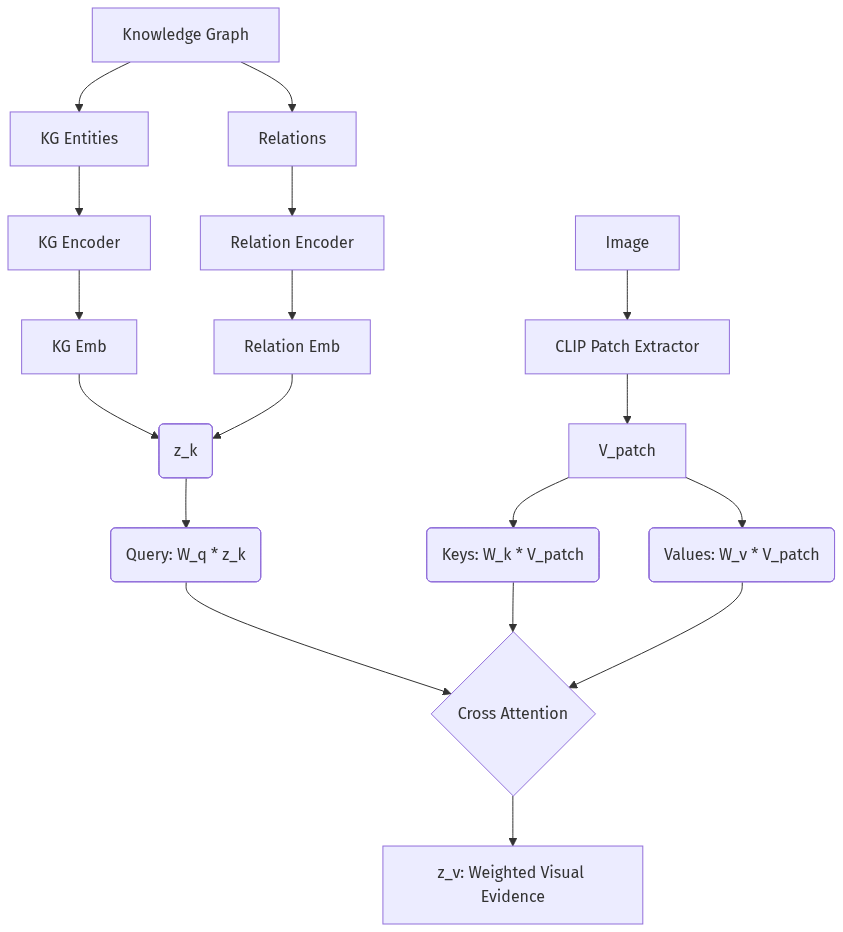
\includegraphics[width=\linewidth]{figures/figure_1_part2_tvcs.png}
    \caption{TVCS module for KG-guided visual evidence extraction.}
    \label{fig:arch_part2}
\end{figure}

\begin{figure}[!htbp]
    \centering
    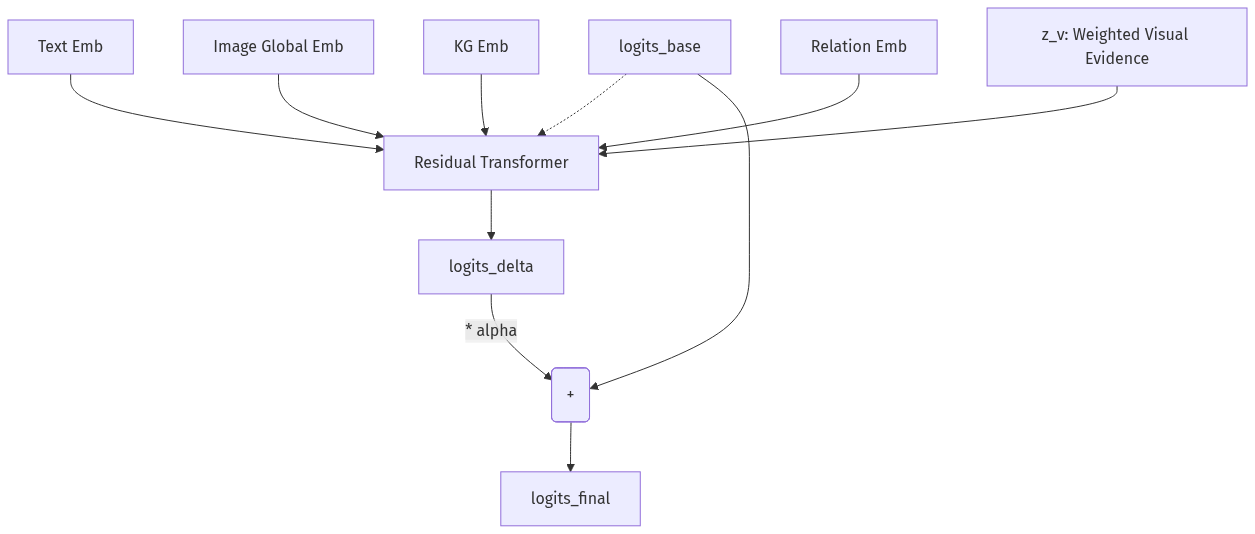
\includegraphics[width=\linewidth]{figures/figure_1_part3_residual.png}
    \caption{Residual Transformer correction and final logit composition.}
    \label{fig:arch_part3}
\end{figure}

The overall data flow across these components can be summarized as follows:
\begin{itemize}
    \item \textbf{Text Input:} Encoded into a text feature using RoBERTa.
    \item \textbf{Image Input:} Encoded into both a global visual feature and fine-grained spatial patch tokens via CLIP.
    \item \textbf{Knowledge Input:} KG entities and relations are encoded into structured representations.
    \item \textbf{TVCS Evidence Extraction:} The TVCS module actively uses the KG/relation representations as a query, attending to CLIP visual patches (key/value) to isolate contradiction signals, producing the rich visual evidence feature $z_v$.
    \item \textbf{Prediction Pipeline:} First, the passive anchor linearly combines text, global image, and KG to produce $\text{logits\_base}$. Then, the Residual Transformer processes $z_v$ (and other modalities) to compute the correction term $\text{logits\_delta}$. The final prediction is formed via residual addition: $\text{logits\_final} = \text{logits\_base} + \alpha * \text{logits\_delta}$. Notably, the final \texttt{no\_c\_emb} model fully removes the scalar class prior (c\_emb) while explicitly preserving the TVCS multidimensional visual evidence $z_v$.
\end{itemize}

The system framework utilizes a passive Text+Image+KG anchor to generate $\text{logits\_base}$. Simultaneously, the TVCS expert module explicitly extracts contradiction evidence ($z_v$) via a cross-attention mechanism.

\subsection{Passive T+I+KG Anchor}
To establish a solid representation foundation, we first set up a passive fusion baseline. The text utterance $T$ is encoded using RoBERTa, while the image $I$ is processed via CLIP to extract both global and patch-level features. The KG entities $K$ and relations $R$ are encoded into continuous vector representations.

In the passive anchor configuration, these modalities are simply concatenated to create a combined multimodal representation. This combined representation is then passed through a fully connected layer to compute the base classification logits ($\text{logits\_base}$). Although this approach integrates knowledge as supplementary context, it lacks the explicit mechanisms required to actively detect intentional contradictions between visual content and the provided knowledge.

\subsection{TVCS: Knowledge-Guided Visual Contradiction Scoring Expert Module}
To overcome the limitations of the passive fusion method, we introduce the TVCS (Knowledge-guided Visual Contradiction Scoring) expert module. The objective of this module is to model explicit interactions between external knowledge and visual components, thereby enabling the detection of multimodal inconsistencies at a fine-grained level.

The TVCS expert module uses a cross-attention mechanism, where the query is derived from KG and relation embeddings ($z_k$), while keys and values are extracted from CLIP visual patches ($V_{patch}$). This architecture allows the model to actively scan the image to find specific patches that support or contradict the provided knowledge claim. The attention operation yields a weighted visual evidence vector, $z_v$:

\begin{align}
    \text{query} &= W_q z_k \\
    \text{keys} &= W_k V_{patch} \\
    \text{values} &= W_v V_{patch} \\
    z_v &= \sum \text{softmax}(\text{query} \cdot \text{keys}^T) \text{values}_i
\end{align}

It is important to note that the evidence $z_v$ derived from TVCS captures visual signals correlated with knowledge inconsistency, acting as a knowledge-grounded inconsistency signal, rather than absolute proof of truthfulness.

\subsection{Residual Transformer Correction}
Instead of replacing the highly stable base classifier, we use the TVCS expert module as a residual correction branch. The derived visual evidence $z_v$, along with the original text features, global image, and KG relations, are processed through a Residual Transformer to compute the correction vector $\text{logits\_delta}$.

The final prediction is then formulated as a residual addition:
\begin{equation}
\text{logits\_final} = \text{logits\_base} + \alpha * \text{logits\_delta}
\end{equation}

This design ensures that the model preserves the generalized discriminative capability of the passive anchor, while dynamically adjusting predictions based on explicit contradiction evidence when necessary.

\subsection{no\_c\_emb Variant}
During the architectural design phase, we initially experimented with integrating a scalar class embedding representation (c\_emb) to directly inject class structure priors. However, empirical analysis (detailed in Section 6) revealed that c\_emb acted as a detrimental "shortcut", encouraging the neural network to overfit based on prior class probabilities rather than genuinely contrasting multimodal evidence.

Consequently, our final proposed architecture is the no\_c\_emb variant. By completely eliminating the scalar quantity c\_emb, we force the model to rely entirely on the high-quality visual evidence $z_v$ derived from TVCS. The TVCS module remains the core, indispensable component in this final architecture.

\subsection{Training Objective and Model Selection}
The model is optimized using a combined loss function, comprising the standard cross-entropy classification loss ($L_{cls}$) and a specialized binary cross-entropy loss for TVCS ($L_{tvcs}$). The TVCS loss is strictly masked and applied exclusively to distinguish between genuine multimodal alignment (Real) and fabricated contradiction samples (CK).

\begin{equation}
L_{total} = L_{cls} + \lambda * L_{tvcs}
\end{equation}

To prevent data leakage and ensure reliable generalization capability, the model checkpoint selection is strictly performed following a validation-only protocol, without any tuning on the test set. All final reported test metrics are obtained from a locked evaluation phase.

